\section{Appendix}

\subsection{Dataset Statistics}

\begin{table}[h]
    \centering
    \caption{Dataset Statistics}
    \label{tab:data}
    \begin{tabular}{lllll}
        \toprule
        & \textbf{Split} & \textbf{\#Samples} (\%) & \textbf{\#Targets} & \textbf{Overlap} \\
        \midrule
        \multirow{3}{*}{\texttt{TM}} 
        & Train. & 65,846 (62\%) & 59 & N/A \\
        & Val. & 15,031 (14\%) & 47 & 10 \\
        & Test. & 25,083 (24\%) & 37 & 4 \\
        \\
        \multirow{3}{*}{\texttt{SP}} 
        & Train. & 12,141 (85\%) & 636 & N/A \\
        & Val. & 1,407 (10\%) & 159 & 0 \\
        & Test. & 703 (5\%) & 89 & 0 \\
        \bottomrule
    \end{tabular}
\end{table}

\subsection{Benchmark Performance}

% \begin{figure*}
    % \centering
    % 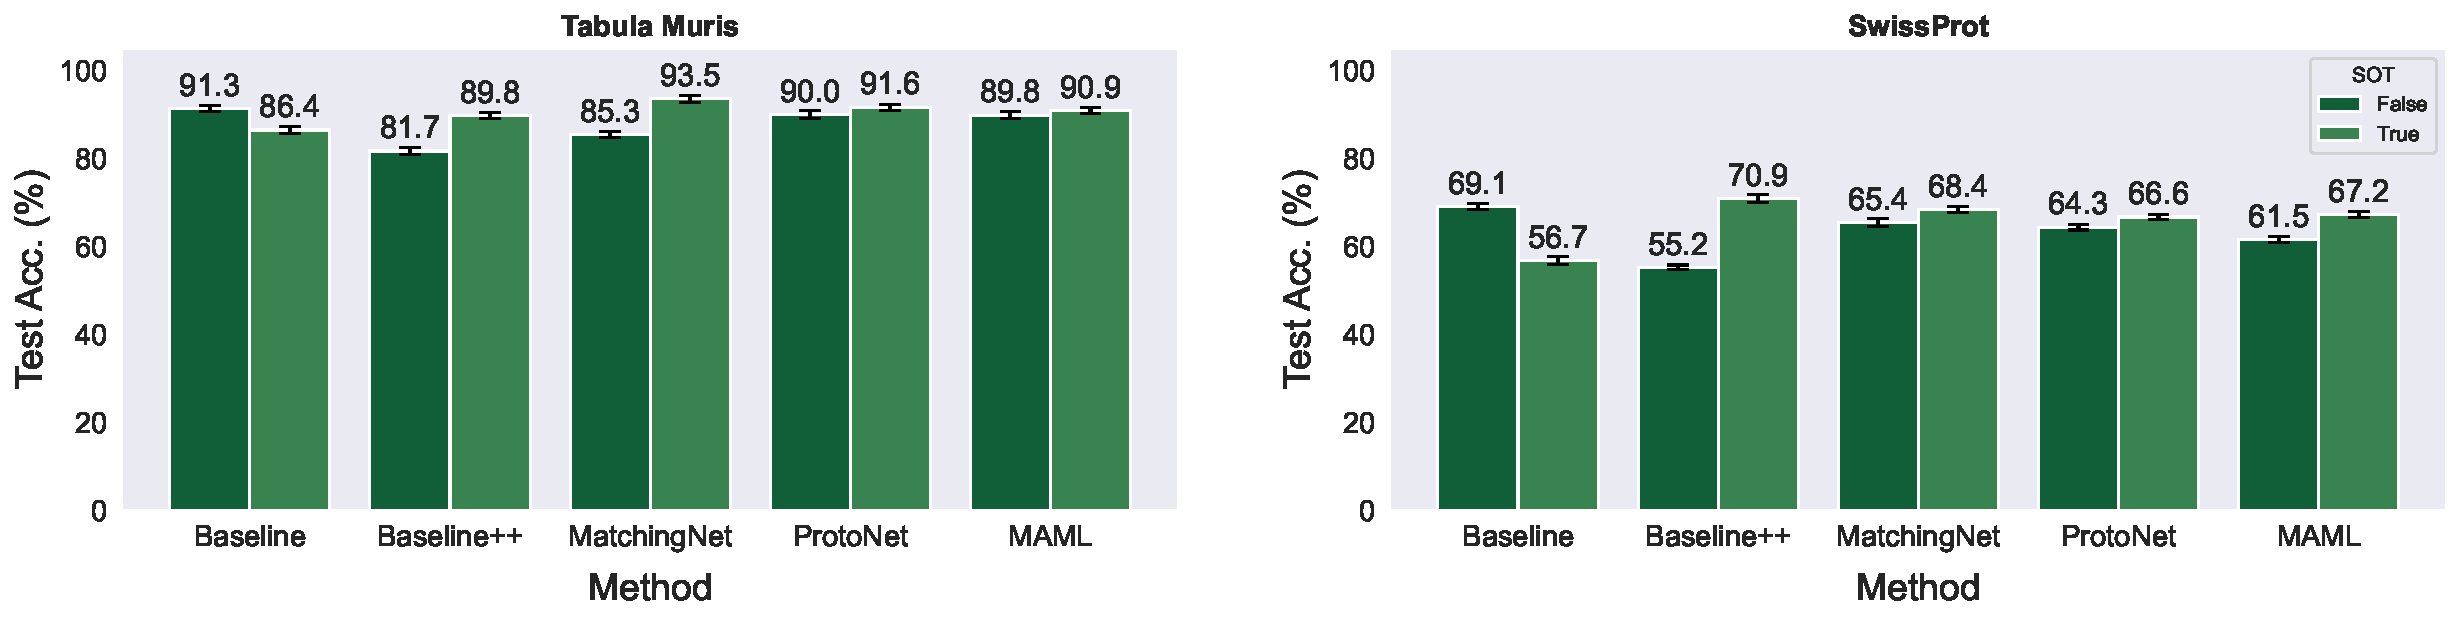
\includegraphics[width=0.9\linewidth]{../figures/benchmark-perf.pdf}
    % \caption{Test accuracy of all methods on \texttt{TM} (left) and \texttt{SP} (right) in the 5-way-5-shot setting.}
    % \label{fig:benchmark-perf}
% \end{figure*}